\chapter{Application implementation}

\section{Architecture considerations}
As a summary of Chapter 2, we can summarize a short comparison between possible architectures:

\begin{enumerate}
    \item Native application
          \begin{itemize}
              \item Requires distribution on multiple marketplaces (Google Play Store, Apple App Store).
              \item Requires multiple builds (for each supported platform: iOS, Android).
              \item Installation necessary.
              \item Internet not required for base functionality.
          \end{itemize}
    \item Web application
          \begin{itemize}
              \item Distribution is straightforward (accessing a link is sufficient).
              \item No installation necessary.
              \item Cross-platform by default.
              \item Internet required for base functionality.
          \end{itemize}
    \item Progressive Web Application
          \begin{itemize}
              \item Distribution is straightforward (accessing a link is sufficient).
              \item No installation necessary, although possible.
              \item Internet not required for base functionality (even if not installed).
          \end{itemize}
\end{enumerate}

Remarks relative to our product requirements (section \ref{sec:Requirements}):
\begin{enumerate}
    \item Our train companion app intends to be easy to use and access. Asking users to download and install a native application goes against this intention.
    \item Our train companion app must work without Internet. Asking users to access a website every time they want to use our application goes against this requirement.
\end{enumerate}

The choice of a Progressive Web Application architecture is therefore justified, since this resolves a series of drawbacks of both other possible architectures.

\section{Entities}
\label{sec:Entities}
By parsing the requirements (section \ref{sec:Requirements}), we can identify a series of entities that the user must interact with:

\begin{enumerate}
    \item Train trip
          \begin{itemize}
              \item A train trip represents a trip defined by a train ticket.
              \item The trip cannot have transfer stops.
              \item A trip has the following properties: train number, departure station, destination station, date, owner (user account). Additional trip information can be deduced from the traffic data (stops, timetable, delays).
          \end{itemize}
    \item User account
          \begin{itemize}
              \item A user account is used to represent a single person using the application.
              \item An account stores the user's preferences.
              \item An account contains a list of social ids, one id for each social login provi\-der (Google, Apple).
          \end{itemize}
\end{enumerate}

In addition, we must recognize that CFR travel information must be stored as well. For this, we can make use of the General Transit Feed Specification, abbreviated GTFS, standard. In particular, we look at the GTFS Schedule variant, which provides static (schedule) information, without live data, and we can obtain the entities that our application needs from there.

From the GTFS Schedule reference, we make use of a subset of entities, enumerated in Table \ref{TableGTFS}. Notably, we omit entities related to fares, station layouts, translations, headways.

We only use a subset of GTFS data because the public traffic datasets that Romanian operators publish only contain data related to this subset, and don't make use of other GTFS features like fares.

\begin{table}[htbp]
    \centering
    \begin{tabular}{|m{0.25\textwidth}|m{.65\textwidth}|}
        \hline
        GTFS filename       & Description                                                                                                          \\
        \hline
        agency.txt          & The railway operators in Romania, which includes the national operator CFR along with a couple of private operators. \\
        \hline
        stops.txt           & All stations.                                                                                                        \\
        \hline
        routes.txt          & Transit routes. A route is a group of trips that are displayed to passengers as a single service.                    \\
        \hline
        trips.txt           & Trips for each route. A trip is a sequence of two or more stops that occur during a specific time period.            \\
        \hline
        stop\_times.txt     & Times that a train arrives at and departs from stops for each trip.                                                  \\
        \hline
        calendar.txt        & Service dates specified using a weekly schedule with start and end dates.                                            \\
        \hline
        calendar\_dates.txt & Exceptions for the services defined in the calendar.txt.                                                             \\
        \hline
    \end{tabular}
    \caption{GTFS Schedule data that we are going to make use of.}
    \label{TableGTFS}
\end{table}

\section{Sourcing of the GTFS travel data}

Although Romanian train operators publish their travel data annually \cite{DataGovRoDespre} \cite{DataGovRoLicense}, the data comes in a monolithic non-standard XML file, that is directly unusable for our application.

We use the GTFS format for our application because it is structured on "tables", is widely supported and is very easily indexable. Therefore, we must find a way to convert this XML data to GTFS.

Thankfully, such a converter already exists, in the form of Vasile Cotovanu's GTFS exporter \cite{VasileRubyExporter} written in Ruby and published on his GitHub account, that has the wonderful handle of \verb|vasile|.

Running the exporter produces a list of text files as detailed in Table \ref{TableGTFS}. Although the data is in a familiar tabular format, it is not easily parsable and indexable in this CSV form. Further processing is detailed in the section pertaining to databases.

\section{Application infrastructure overview}

\begin{figure}[htbp]
    \centering
    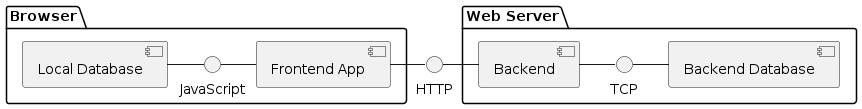
\includegraphics[width=\textwidth]{./figures/ch4_component-diagram.png}
    \caption{Generic component diagram for our application, with no specific software in mind.}
    \label{FigGenericComponentDiagram}
\end{figure}

Based on the requirements in Section \ref{sec:Requirements} and entities defined in Section \ref{sec:Entities}, it is useful to lay out how the infrastructure of the application is laid. One observation to be made about our requirements is how we need to store data both locally on the user's device, and in the cloud. Therefore, an architecture resembling Figure \ref{FigGenericComponentDiagram} must be set up, to allow this separation of data storage.

In the following sections, we discuss different software options we can use to build out this infrastructure.

\section{Databases}
The plural is intentional, since we need to decide on how the databases for both the frontend and the backend will look.

It is useful to start by analyzing what kind of data is necessary in which side, how much data exists in each side, and how often it will be accessed.

\subsection{Frontend database}
The question of where to store the GTFS travel information is one that easily finds its answer in the frontend database, for the simple reason that the requirements (Section \ref{sec:Requirements}) mandate that this travel information be available offline.

Having the GTFS travel data available offline brings a number of advantages, such as:
\begin{enumerate}
    \item Accessing the data is blazing fast and not subject to (extremely variable) network latency.
    \item A step of abstraction, in the form of an Internet API, is not needed, reducing complexity.
\end{enumerate}

Conversely, storing the data offline is disadvantageous because:
\begin{enumerate}
    \setcounter{enumi}{2}
    \item There might not be suitable browser functionality to store this data with.
    \item The dataset might be too large to store.
    \item The dataset might take too long to download.
\end{enumerate}

However, these disadvantages (and potential disadvantages) can be mitigated using the following methods (and arguments):
\begin{enumerate}
    \setcounter{enumi}{5}
    \item \textbf{(For 3)} A suitable place to store large amounts of data \textit{does} exist, in the form of IndexedDB \cite{IndexedDBIntro}.
    \item \textbf{(For 4)} The IndexedDB quotas easily fit around the size of our GTFS dataset \cite{IndexedDBLimits}.
    \item \textbf{(For 5)} Mitigating long download times is not wholly possible, but we can make the user aware of when travel data is downloading, and implement caching strategies both client-side and server-side, to alleviate this issue.
\end{enumerate}

We also need to store trip history information in the user's browser. Although this can easily be accomplished using other storage methods such as Local Storage, we already made use of IndexedDB, therefore we can just create a separate database to the GTFS data and store our trip history there.

As part of our caching strategy for the disadvantage of number 5 mentioned above, we also need to store when the last travel data was downloaded.

A diagram of this architecture can be viewed in Figure \ref{FigDbDiagram}.

\subsection{Backend database}
The backend is only needed to authenticate users and to store trip history for them. Therefore, we do not expect database traffic to need to be distributed across the world or be particularly efficient, since database calls are expected to be few and far in-between.

As such, I chose MySQL for this purpose, since it is easy to set up and does not require extensive configuration.

This database needs to store a list of users, and a list of trips.


A diagram of the architectures of both backend and frontend databases is shown in Figure \ref{FigDbDiagram}.

\begin{figure}[htbp]
    \centering
    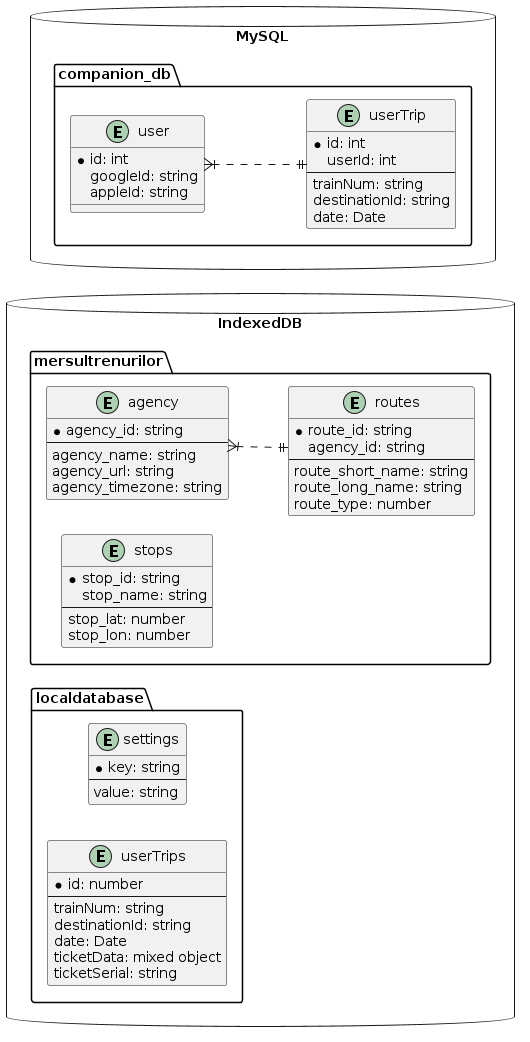
\includegraphics[width=0.7\textwidth]{./figures/ch4_db-diagram.png}
    \caption{Database diagram of both databases.}
    \label{FigDbDiagram}
\end{figure}

\section{Frontend tech stack}
The use of client-side JavaScript cannot be ruled out since this is an application that needs to run offline, therefore solutions involving server-rendered pages (PHP, ASP, JSP).

We must then look to UI frameworks the likes of React, Angular, or Vue. Each UI framework has advantages and disadvantages, but I chose React since it is more lightweight and has more support in the JavaScript ecosystem.

Since we're working with JavaScript, we have a choice to make between working with plain JavaScript, or configuring TypeScript to aid in compile-time safety. There are good arguments to use either, but I went with TypeScript because I am very proficient with it.

Working with IndexedDB can be done using the native browser APIs